%\part{Konstruktion}

\chapter{User Interface}

Im Folgenden wird ein Überblick über die Klassenabhängigkeiten des User Interfaces gegeben, der Ablauf bei der Anzeige eines \SEARCH-Links erklärt sowie die Packagebedeutungen innerhalb des User Interfaces erläutert.

\begin{figure}[h]
	\centering
	\includegraphics[width=\textwidth]{UI_Uebersicht_Klassenabhaengigkeiten}
	\caption{Klassenabhängigkeiten im UI}
\end{figure}

Die obige Darstellung zeigt die Verbindungen der Klassen des User Interfaces. Hierbei steht der \lstinline|ViewController| im Mittelpunkt, da von ihm die meiste Funktionalität ausgeht.

\begin{figure}[ht]
	\centering
	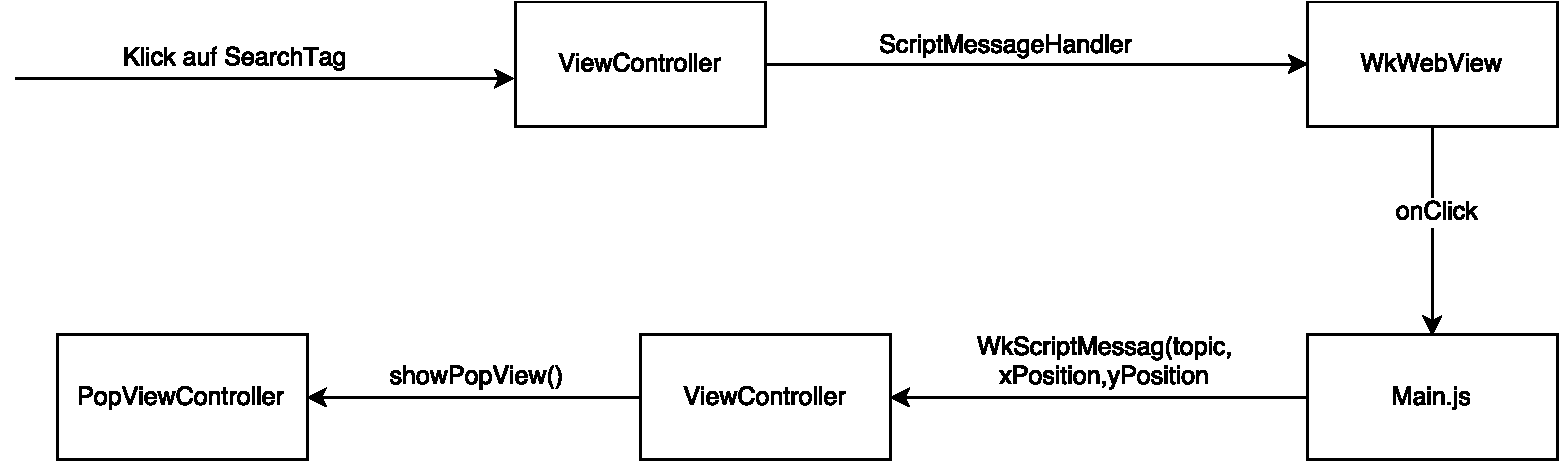
\includegraphics[width=\textwidth]{SearchTagAnzeige}
	\caption{Searchtag Anzeige}
\end{figure}

Obige Grafik zeigt den Programmablauf nach dem Tippen auf einen \SEARCH-Tag. Die Position des Tipps wird über JavaScript ausgelesen und an den \lstinline|WkWebview| weitergeleitet. Dieser erzeugt an der übertragenen Position einen \lstinline|PopView| und zeigt diesen an. 

%\part{Konstruktion}
%\chapter{User Interface}

\section{ViewController}
Der ViewController dient zur Steuerung der Funktionen welche direkt mit dem Interface zusammen gehören. Dazu gehören
IBActions welche von Buttons oder anderen Interkationsflächen angestoßen werden können, sowie Funktionen welche direkt mit diesen zusammenhängen, Beziehungsweise aus diesen resultieren. Der ViewController ist die zweite Schicht nach dem UI. Im
Folgenden werden die einzelnen Viewcontroller mit ihren jeweiligen Funktionen beschrieben.
Der Viewcontroller ist der Hauptviewcontroller für die normale Browseransicht mit der Adresszeile und dem WkWebView. Er verwaltet die Kopzeile mit Adresszeile sowie den Buttons für Vorwärts, Zurück, Lesezeichen, Lesezeichen hinzufügen, Reload, Sech-Tabelle sowie die Settings. Die datei Main.js welche aus dem Viewcontroller heraus aufgerufen wird, markiert alle gefundenen Search-Tags. Außerdem wird im Falle eines Klicks die Position sowie die id des Search-Tags übermittelt.
Der PopViewController ist zuständig für die Verwaltung eines neuen PopViews, beim klicken auf einen Searchtag. Er verwaltet die Anzeige des ausgewählten Searchlinks in einem neuen WkWebView sowie den Button für die Auswahl der verschiedenen Suchergebnisse zu einem Searchtag.
Der SearchTableViewController verwaltet die einzellnen Suchergebnisse zu einem Searchtag. Alle Ergebnisse werden sortiert in einer Tabelle mit Bild, Title und Link angezeigt.
Der Settingscontroller is für die verwaltung der Browsereinstellungen zuständig.
\subsection{ViewController}
\subsection{SearchTableViewController}
\subsection{PopViewController}
\subsection{SettingsController}
\subsection{main.js}
\subsection{readHead.js}

%\subsubsection{Unterteilabschnitt}
%\paragraph{Paragraph}
%\subparagraph{Unterparagraph}

\newpage
%\part{Konstruktion}
%\chapter{User Interface}

\section{Delegate}

Die Delegates im \SECH-Browser dienen zur Bereitstellung einer einheitlichen Struktur innerhalb des Programms. Von den einzelnen Delegate Klassen werden Funktionen zur Darstellung von Informationen oder interne Protokolle aufgerufen. Im \lstinline|WebViewDelegate| werden die Funktionen zur Validierung der Website mit Hilfe der JavaScript Dateien und die Extraktion der \SEARCH-Tags angestoßen.

Die \lstinline|readHead.js| enthält den Javascript Code zur Auslesen des Headbereiches einer HTML-Seite. In der Klasse \lstinline|FavTableDelegate| werden die Lesezeichen bereitgestellt. Der Benutzer hat die Möglichkeit ein ausgewähltes Lesezeichen auszuwählen und es sich im Browser anzeigen zulassen. Zusätzlich enhält die Klasse die Funktionen, um Lesezeichen bearbeiten und löschen zu können. Der SechTableDelegate enthält die Routine zum Darstellen von \SEARCH-Links aus der \SECH-Tabelle. 
\subsection{AppDelegate}
\subsection{WebViewDelegate}
\subsection{readHead.js}
\subsection{FavTableDelegate}
\subsection{SechTableDelegate}

%\subsubsection{Unterteilabschnitt}
%\paragraph{Paragraph}
%\subparagraph{Unterparagraph}

\newpage
%\part{Konstruktion}
%\chapter{User Interface}

\section{DataSource}
Die DataSources im \SECH-Browser dienen zur Bereitstellung der Daten in den Tabellen. Von den einzelnen Klassen werden jeweils Funktionen zum befüllen der einzelnen Zellen aufgerufen. In der Klasse FavTableDataSource werden zunächst alle gespeicherten Lesezeichen geladen, anschließend werden die einzelnen Zellen der Tabelle mit den Lesezeichen befüllt. Im SechTableDataSource werden alle \SEARCH-Tags die auf der Seite gefunden wurden in den Zellen der \SECH-Tabelle dargestellt. Zusätzliche befinden sich noch Funktionen zum Erweitern der \SEARCH-Tags in der Klasse.

\subsection{FavTableDataSource}
\subsection{SechTableDataSource}

%\subsubsection{Unterteilabschnitt}
%\paragraph{Paragraph}
%\subparagraph{Unterparagraph}


\newpage
%\part{Konstruktion}
%\chapter{User Interface}

\section{Components}

In den Components werden die spezifischen Zellen für die Lesezeichen-Tabelle und Search-Tag-Tabelle modelliert, die in den jeweiligen Delegates verwendet werden. Weiterhin ist in Components die Validierung für die AddressBar definiert, welche die Eingaben in der Suchleiste überprüft und verwaltet.

\newpage
%\part{Konstruktion}
%\chapter{User Interface}
%\section{Packages}

\subsection{Persistence}
Im Persistence-Package befinden sich Models die für eine persistente Speicherung gedacht sind. Das \lstinline|FavouritesModel| stellt einerseits das nötige Model, andererseits die Funktion für das Speichern von Lesezeichen zur Verfügung.
\newpage
%\part{Konstruktion}
%\chapter{User Interface}

\section{WebContent}

Der \lstinline|WebContent| stellt die Schnittstelle zwischen dem UI und der SearchExtraction dar. Er beinhaltet HTML-Code, in Form eines Strings, sowie die URL, von welcher der HTML-Code stammt. Der HTML-Code ist in den Head und den Body der Website aufgeteilt.\newline
Aus dem \lstinline|WebContent| wird in der SearchExtraction ein \lstinline|SearchModel| erzeugt.

%\subsection{Teilabschnitt}
%\subsubsection{Unterteilabschnitt}
%\paragraph{Paragraph}
%\subparagraph{Unterparagraph}


